\documentclass[xetex,svgnames]{scrartcl}

% packages
\usepackage{xltxtra}
\usepackage{polyglossia}
\usepackage{lsalike}
\usepackage{hyperref}
\usepackage{fontspec}
\usepackage{covington}
\usepackage{scrpage2}
\usepackage{qtree}
\usepackage[left=2cm,right=2cm,top=3cm,bottom=3cm]{geometry}
\usepackage{draftwatermark}
\usepackage{hieroglf}
\usepackage[weather,misc,alpine]{ifsym}
\usepackage{phaistos}
\usepackage{linearb}
\usepackage{dingbat}
\usepackage{pst-node}
\usepackage{colortbl}
\usepackage{alltt}
\usepackage{listings}

% fonts general
\setmainfont[Mapping=tex-text,Scale=1.0]{FreeSans}
\setsansfont[Mapping=tex-text,Scale=1.0]{FreeSans}
\setmonofont{FreeMono}

% special fonts
\newfontfamily\hana{HAN NOM A}
\newfontfamily\hanb{HAN NOM B}
\newfontfamily\sil{Doulos SIL}
\newfontfamily\grk{Aristarcoj}
\newfontfamily\calligraphy{Chinese Calligraphy}
\newfontfamily\jin{cjkbronze}
\newfontfamily\jiagu{cjkjiagu}
\newfontfamily\xiaozhuan{shuowenxiaozhuan}
\newfontfamily\pur{Purisa}
\newfontfamily\cjcalligraphy{sinocalligraphy}

% specific commands
\newcommand{\mysub}[1]{\raisebox{-0.5ex}{\scriptsize{#1}}}
\SetWatermarkText{PYTHON}
\newcommand{\bild}[2]{%
    \scalebox{#1}{%
        \includegraphics{/home/mattis/projects/graphics/img/#2.jpg}
        }
    }
\newcommand{\Table}[1]{%
    \begin{flushleft}
        \begin{tabular}{|p{16.5cm}|}
            \hline \cellcolor{lightgray} \bf \pur #1
            \\\hline
        \end{tabular}
    \end{flushleft}
}

\lstset{language=Python}

\newcommand{\Code}[1]{%
    \begin{flushleft}
        \begin{tabular}{||p{16.5cm}||}
            \hline\hline \cellcolor{white}
            \\
            #1

             \cellcolor{white}
            \\\hline\hline
        \end{tabular}
    \end{flushleft}
}
\newcommand{\White}[1]{\cellcolor{white} \textcolor{black}{ #1}}

% language settings
\setmainlanguage[spelling=new]{german}
\setotherlanguage{english}

% pagestyle settings
\pagestyle{scrheadings}
\ihead{Johann-Mattis List}
\chead{Python und JavaScript}
\ohead{Aufgabe 2}
\ifoot{}
\cfoot{\pagemark}
\ofoot{}

\newcommand{\Rabbit}[1]{%
\tabular{c}
\scalebox{0.2}{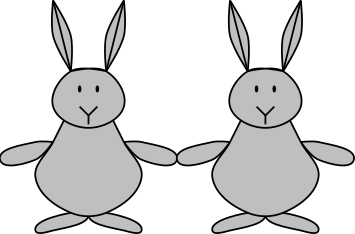
\includegraphics{/home/mattis/projects/graphics/pstricks/rabbits/rabbits.pdf}}\\
#1
\endtabular}

\begin{document}
%\maketitle
\begin{center}
    {\textcolor{Crimson}{\bf \huge  Fibonaccis Kaninchen} }
\end{center}
\section*{\textcolor{Crimson}{Ausgangslage} }
Die Zahlenfolge [0, 1, 1, 2, 3, 5, 8, 13, \ldots] verdankt ihre Berühmtheit dem
italienischen Mathematiker Leonardo Fibonacci (ca. 1180 — 1241), der sie im
Jahre 1202 verwendete, um das Wachstum von Kaninchenpopulationen zu
beschreiben. Fibonacci legte folgende Annahmen zugrunde (entnommen aus:
\url{http://de.wikipedia.org/wiki/Fibonacci-Folge}):
\begin{enumerate}
    \item Jedes Paar wirft pro Monat ein weiteres Paar Kaninchen.
    \item Ein neugeborenes Paar bekommt erst im zweiten Lebensmonat Nachwuchs
        [\ldots].
    \item Die Tiere befinden sich in einem abgeschlossenen Raum [\ldots], so
        dass kein Tier die Population verlassen und keines von außen
        hinzukommen kann.
\end{enumerate}
Die folgende Abbildung verdeutlicht, wie die Anzahl der Kaninchenpärchen im
Laufe der Monate anwächst.
\begin{center}
    \scalebox{0.8}{
    \begin{psmatrix}[colsep=0.2,rowsep=0.5]

    \psframebox{\bf 0}
    \\
    [name=a] \psframebox{\bf 1} & 
     &
     [name=1] \Rabbit{1} \\ 
    [name=b]\psframebox{\bf 2} &  &
    [name=12] \Rabbit{1} \\ 
    [name=c]\psframebox{\bf 3} &  &
    [name=13]\Rabbit{1} & &&&&[name=2] \Rabbit{2} \\
    [name=d]\psframebox{\bf 4} &  &
    [name=14] \Rabbit{1} &&&[name=3]\Rabbit{3} &&[name=21]\Rabbit{2} \\
    [name=e]\psframebox{\bf 5} &  & [name=15]\Rabbit{1} &&
    [name=4]\Rabbit{4} & [name=31] \Rabbit{3} &&[name=5] \Rabbit{2} &&
    [name=22]\Rabbit{5} \\ 
    [name=f]\psframebox{\bf 6} &  & [name=16]
    \Rabbit{1} & [name=6] \Rabbit{6} & [name=41] \Rabbit{4} &
    [name=32] \Rabbit{3} & [name=7] \Rabbit{7} & [name=51]
    \Rabbit{2} & [name=8] \Rabbit{8} & [name=23] \Rabbit{5} &\\
    
    
    \ncline{1}{12}
    \ncline{12}{13}
    \ncline{13}{14}
    \ncline{14}{15}
    \ncline{15}{16}
    \ncline{2}{21}
    \ncline{21}{22}
    \ncline{22}{23}
    \ncline{23}{24}
    \ncline{24}{25}
    \ncline{25}{26}
    \ncline{3}{31}
    \ncline{31}{32}
    \ncline{33}{34}

    \ncline{4}{41}
    \ncline{41}{42}
    \ncline{12}{2}
    \ncline{13}{3}
    \ncline{14}{4}
    \ncline{15}{6}
    \ncline{21}{5}
    \ncline{5}{8}
    \ncline{31}{7}
    \ncline{5}{51}

\end{psmatrix}
}
\end{center}
\section*{\textcolor{Crimson}{Aufgabe 1} }
\Table{Schreiben Sie eine Funktion (<fibonacci()>), welche rekursiv die Anzahl von
Kaninchenpärchen in einem bestimmten Monat berechnet. Bei einer Eingabe von
{\bf 4} (also 4 Monaten) würde diese Funktion, wie man aus der Graphik ablesen
kann, die Zahl 3 zurückgeben. Informieren Sie Sich
gegebenenfalls im Internet oder in anderen Quellen genauer darüber, wie eine solche Funktion in Python
geschrieben werden kann, wobei im Falle einer durchgängigen Übernahme fremden
Quellcodes die Quelle angegeben werden sollte. Wenden Sie das Programm, falls es
funktioniert, auf einige Versuchszahlen an und erläutern Sie im Quellcode (in
Kommentarform), worin eventuelle Nachteile einer puren rekursiven Lösung einer
solchen Aufgabe liegen.}
\section*{\textcolor{Crimson}{Aufgabe 2}}
\Table{Wir schreiben das Jahr 2018. Nachdem kurz nach dem erfolgreichen Abschluss
Ihrer Bachelor/Masterprüfung mit Bestnoten ein kleines Software-Startupunternehmen 
(HHUD Pythonics) Ihre Qualitäten als Programmierer erkannt und Sie umfangreich
gefördert hat, sind Sie
inzwischen für eine Ablösesumme von 1000000 D-Mark zu Google gewechselt. Dort
weht Ihnen jedoch ein ganz anderer Wind entgegen, als sie das von der HHUD
Pythonics gewohnt waren. Insbesondere Ihre rekursive Fibonacci-Lösung
(<fibonacci.py>) zur Berechnung der Wachstumsraten von Kaninchenpopulationen
wird von dem Unternehmen als nicht mehr zeitgemäß angesehen, da eine
interaktive Abfrage von Zahlen bei Google die Prozessorfarmen des Unternehmens
übermäßig belastet. Sie werden daher unter Androhung einer sofortigen Kündigung 
aufgefordert, innerhalb von einer Woche eine alternative Lösung zu
schaffen, die es den Kaninchenzüchtern unter den Googlenutzern ermöglicht, zu
jedem Zeitpunkt und so schnell wie möglich den Stand ihres Kaninchenbesitzes
abzufragen und abzuwägen, und zwar nicht mehr in Python, sondern als interaktive Applikation in
JavaScript!
 
Sie haben auch schon eine Idee, wie Sie das Ganze
realisieren wollen: Eine rekursive Lösung zäumt die Zahlenreihe von hinten auf.
Was aber nun, wenn man die Zahlenreihe einfach bis zu der entsprechenden Zahl
iterativ berechnet? Die Reihe könnte man darüber hinaus einfach in einem dieser fiesen
JavaScript-Arrays
speichern...
 
Aber die Zeit drängt, und mit jedem Ticken des Sekundenzeigers Ihres
Nostalgieweckers spüren Sie, wie der Druck ansteigt...
}
\end{document}

